\documentclass[12pt]{article}
\usepackage[english,greek]{babel}
\usepackage[utf8x]{inputenc}
\usepackage{graphicx}
\begin{document}


\title{Έγγραφο Απαιτήσεων Λογισμικού \\ Eταιρία Kατασκευής Λογισμικού}
\date{\today}
\author{$Javengers$}
\maketitle

\tableofcontents

\section{Εισαγωγή}

\subsection{Ταυτότητα-Επιχειρησιακοί Στόχοι}

Κύριος στόχος της επιχείρησής μας αποτελεί η διευκόλυνση και εκλέπτυνση της εμπειρίας των αγορών προσφέροντας τη δυνατότητα στους καταναλωτές να εντοπίζουν αποτελεσματικά τα μαγαζιά με τις συμφέρουσες τιμές στα προϊόντα που τους ενδιαφέρουν. Το παραπάνω θα επιτευχθεί μέσω της ανάπτυξης ενός παρατηρητηρίου τιμών που βασίζεται στη μέθοδο του crowdsourcing. Συγκεκριμένα, οι εθελοντές θα έχουν την δυνατότητα να καταγράφουν και να μοιράζονται τις τιμές από διάφορα καταστήματα μέσω της διαδικτυακής μας υπηρεσίας, δημιουργώντας ένα πλούσιο “τιμοκατάλογο” για μια πληθώρα προϊόντων.

\subsection{Περίγραμμα Επιχειρησιακών Λειτουργιών}

Η δική μας επιχείρηση, εκφρασμένη και μέσω του ρόλου του διαχειριστή, θα είναι υπεύθυνη για τη συντήρηση και την επίβλεψη του λογισμικού, καθώς και της αλληλεπίδρασης με τους χρήστες. Στο πλαίσιο αυτό, ο διαχειριστής θα δέχεται αιτήματα από τους χρήστες σχετικά με τη λειτουργία της σελίδας και αν κρίνεται αναγκαίο θα πραγματοποιούνται οι κατάλληλες διαρθρωτικές ενέργειες, ενώ επίσης θα πραγματοποιούνται ανά τακτά χρονικά διαστήματα, μπορούμε να υποθέσουμε κάθε μήνα, έλεγχοι της εύρυθμης λειτουργίας της σελίδας. Έτσι, είναι πιθανό να απαιτείται η λήψη συγκεκριμένων δράσεων για την βελτίωση της σελίδας ή ενδεχομένως την προσθήκη νέων χαρακτηριστικών. Με βάσει την παραπάνω λεκτική περιγραφή, οδηγούμαστε στο ακόλουθο πιο παραστατικό διάγραμμα $UML$.

\begin{center}
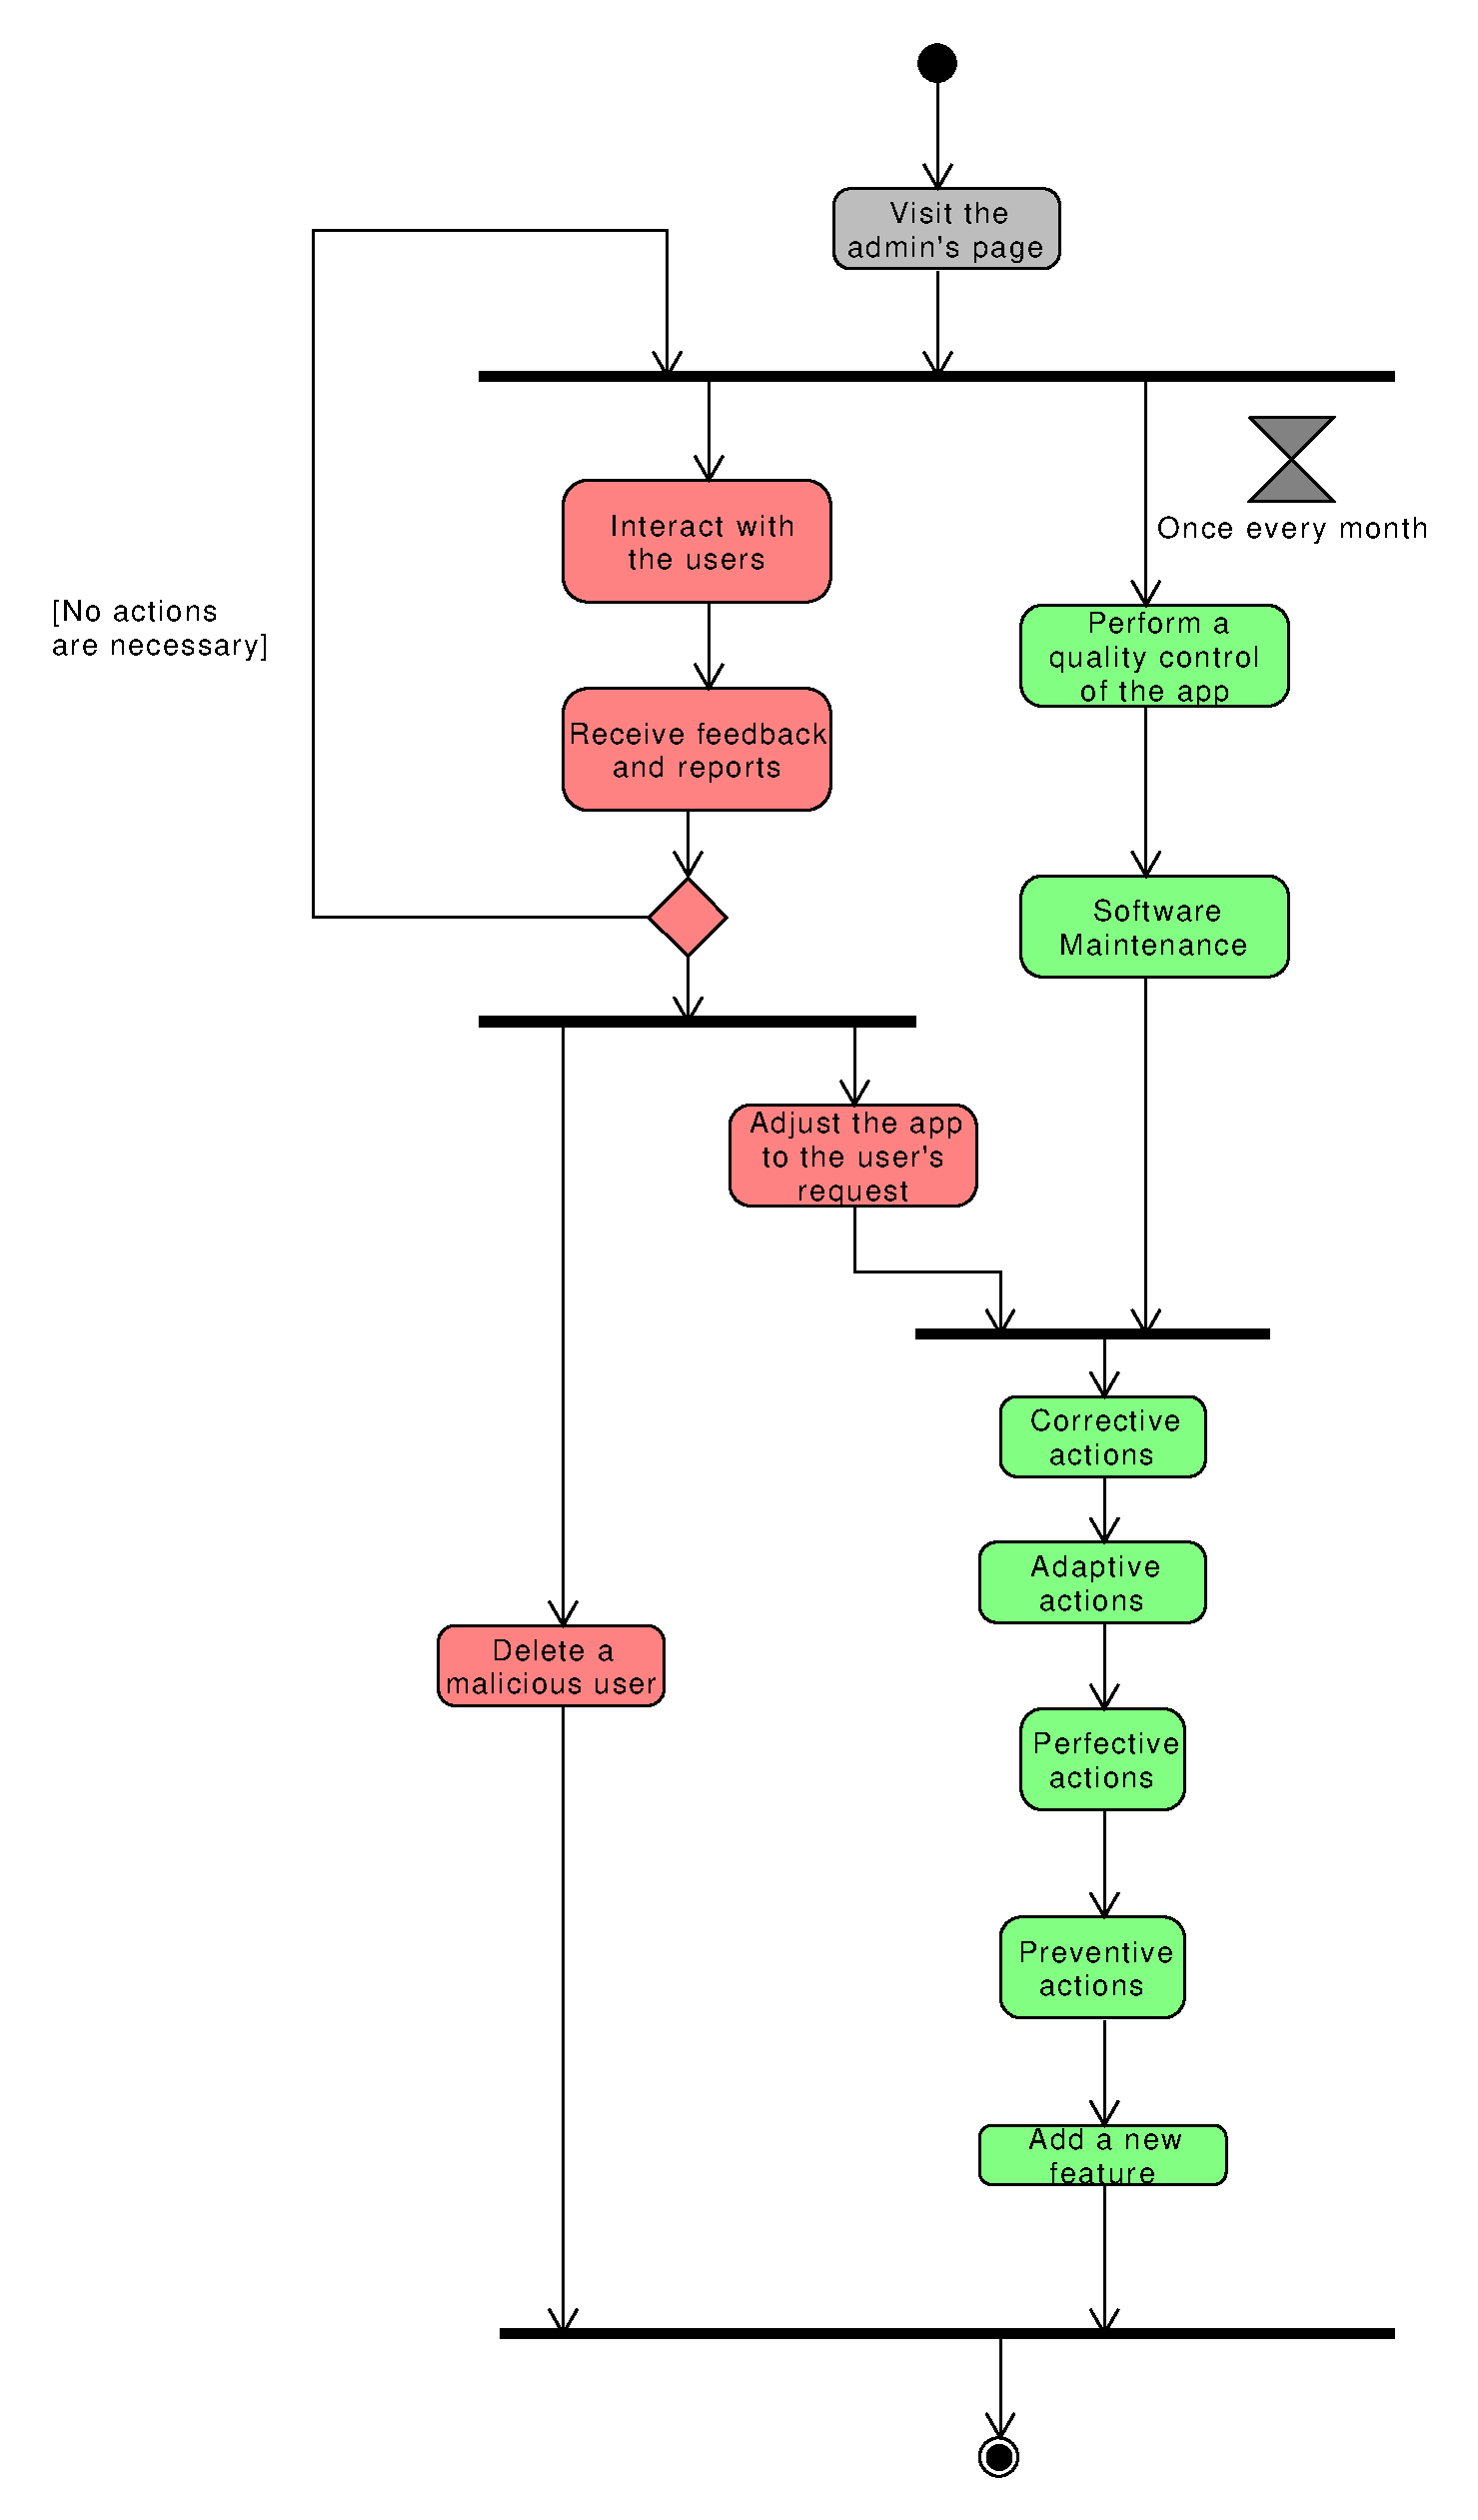
\includegraphics[scale=0.45]{adminActivityDiagram.pdf}
\end{center}


\section{Αναφορές-Πηγές Πληροφοριών}

Η βασική πηγή πληροφοριών για την εφαρμογή μας θα είναι οι αναφορες και οι αξιολογήσεις από τους χρήστες, σχετικά με την λετουργία της σελίδας. Κατ' αυτόν τον τρόπο, καθίσταται δυνατή η αναπροσαρμογή της σελίδας, ωστε να ανταποκρίνεται σε μεγαλύτερο βαθμό στις ανάγκες των χρηστών και να βελτιώνεται η συνολική εμπειρία των χρηστών. 

\section{Διαχειριστικές Απαιτήσεις Επιχειρησιακού Περιβάλλοντος}

\subsection{Επιχειρησιακό Μοντέλο}

Το επιχειρησιακό μοντέλο της επιχείρησής μας συνοψίζεται στα ακόλουθα σημεία:

\begin{itemize}
\item Κύριες Δραστηριότητες: 
	\begin{itemize}
	\item Ανάπτυξη διαδικτυακής πλατφόρμας
	\item $Marketing$-Διαφήμιση
	\item Συντήρηση λογισμικού
	\end{itemize}

	\item Κύριοι Συνεργάτες:
	\begin{itemize}
	\item Ιδιώτες και επιχειρήσεις που εθελοντικά συνεισφέρουν οικονομικά
	\item Εθελοντές του $crowdsourcing$ που προσφέρουν πληροφορίες στην πλατφόρμα μας
	\item Άλλες επιχειρήσεις με τις οποίες η εφαρμογή μας αλληλεπιδρά, όπως είναι το $Google$ $Maps$ $API$ 
	\end{itemize}		
	\item Κύριες Πηγές:
	\begin{itemize}
	\item $Virtual$ $Machine$ που φιλοξενεί τη βάση δεδομένων της σελίδας
	\item $Web$ $Server$
	\item $Human$ $Resources$, δηλαδή όλα τα άτομα που εμπλέκονται στην ομαλή λειτουργία της εφαρμογής
	\end{itemize}
	\item Πρόταση Αξίας:
	\begin{itemize}
	\item Απόδοση
	\item Αξιοπιστία
	\item Ασφάλεια
	\item Εύκολη πρόσβαση σε προσφορές και δυνατότητα σύγκρισης τιμών ανάμεσα σε μεγάλο πλήθος καταστημάτων
	\end{itemize}

	\item $Customer$ $Relations$: 
	\begin{itemize}
	\item $Word$ $of$ $mouth$ 
	\item Διαφημίσεις
	\item Μέσα κοινωνικής δικτύωσης 
	\item Εμφάνιση στις μηχανές αναζήτησης
	\item Υποστήριξη προϊόντων	
	\end{itemize}		
	\item $Channels$:
	\begin{itemize}
	\item $World$ $Wide$ $Web$
	\end{itemize}
	\item $Market$ $and$ $Customer$ $Segments$:
	\begin{itemize}
	\item  Σύνολο των καταναλωτών που έχουν πρόσβαση στο ίντερνετ
	\end{itemize}	 

	\item $Cost$ $structure$: 
	\begin{itemize}
	\item $Marketing$-Διαφημίσεις
	\item Κόστος διατήρησης πλατφόρμας
	\item Νόμιμα $fees$
	\end{itemize}		
	\item $Revenue$ $streams$: 
	\begin{itemize}
	\item Δωρέες από χρήστες που επισκέπτονται της σελίδα μας
	\item Κρατικά και Διακρατικά προγράμματα χρηματοδότησης εφαρμογών.
	\end{itemize}


\end{itemize}


\subsection{Περιβάλλον Διαχείρισης Πληροφοριών}

Την παρούσα χρονική περίοδο, δεν συναντάται αντίστοιχη πλατφόρμα καταγραφής προϊόντων που να βασίζεται στη μέθοδο του πληθωπορισμού. Υπάρχουν φυσικά εταιρίες, όπως είναι το $Skroutz$ που παρέχουν παρόμοιες υπηρεσίες αναζήτησης, ωστόσο βασίζονται σε μεγάλο βαθμό στη συνεργασία με κατασήματα και όχι μεμονωμένα με εθελοντές-χρήστες. Η δική μας εφαρμογή, από την άλλη καλύπτει ένα κενό της αγοράς, ενώ αξίζει να αναφερθεί, ότι ο εθελοντικός της χαρακτηρας ενισχύει την διαφάνεια, την αξιοπιστία και την αμεροληψία των καταχωρήσεων καθώς και την ποικιλία των καταστημάτων, σε σχέση με τις πιο παραδοσιακές προσεγγίσεις που ενδεχομένως ευνοούν τα μεγάλα καταστήματα που έχουν να διαθέσουν μεγαλύτερο κεφάλαιο στη διαφήμιση, έναντι μικρότερων και αναπτυσσόμενων μαγαζιών.

\section{Λειτουργικές απαιτήσεις επιχειρησιακού περιβάλλοντος}

\subsection{Επιχειρησιακές διαδικασίες}

Η συλλογή και εισαγωγή προϊόντων στη βάση δεδομένων θα βασίζεται στο $barcode$.  Συγκεκριμένα, αφού ο χρήστης προσθέσει την τιμή και το τοποθεσία του καταστήματος μέσω της εφαρμογής $Google-Maps$, θα χρησιμοποιείται το $barcode$ ώστε να γίνει αναζήτηση σε μια βάση δεδομένων που θα πραγματοποιεί την ταυτοποίηση του . Στην περίπτωση που η συγκεκριμένη καταχώρηση δεν ταυτοποιηθεί, ο χρήστης καλείται να προσθέσει επιπρόσθετες πληροφορίες, όπως είναι η κατηγορία, ο κατασκευαστής και το όνομα και με βάσει αυτές τις τιμές ενημερώνεται και αντίστοιχη βάση δεδομένων ταυτοποίσης.

\subsection{Περιορισμοί}

Η εφαρμογή μας περιορίζεται από τα δεδομένα που εισάγουν ατομικά οι εθελοντές, ανεξάρτητα από το αντίστοιχο κατάστημα ή την επιχείρηση. Ο συγκεκριμένος περιορισμός, μάλιστα, μας διαχωρίζει από τα παραδοσιακά παρατηρητήρια τιμών που συνεργάζονται συνήθως με μεγάλες αλυσίδες καταστημάτων. Επιπλέον, χρησιμοποιώντας μεθόδους κρυπτογράφησης καθώς και το πρωτόκολλο $https$, αποκρύπτονται οι ευαίσθητες πληροφοριές των χρηστών, όπως είναι ο κωδικός πρόσβασης και ο αριθμός τηλεφώνου. 


\subsection{Δείκτες ποιότητας}

Για να κριθεί η ποιότητας της εφαρμογής πρέπει να λάβουμε υπ' όψη διάφορες παραμέτρους. Τα κύρια σημεία είναι τα ακόλουθα:
	
\begin{itemize}
		\item Η απόδοση του συστήματος	ώστε να εξασφαλίζεται ταχεία πλοήγηση
		\item Ασφάλεια των ευαίσθητων δεδομένων των χρηστών που αφορούν προσωπικά δεδομένα με τη χρήση μεθόδων κρυπτογράφησης. Συγκεκριμένα, θα χρησιμοποιούνται συναρτήσεις κατακερματισμού και η μέθοδος $SHA-3$
	\item Αξιοπιστια και διαθεσιμότητα του συστήματος, ώστε να εξασφαλίζεται ακεραιότητα και αδιάκοπη παροχή υπηρεσιών
	\item Φιλικό και προσαρμοστικό προς το χρήστη $UI$, προσφέροντας απλότητα και ευκολία στην πλοήγηση
	\item Το πλήθος των εγγεγραμμένων χρηστών
	\item Το πλήθος των συνολικών επισκεπτών της σελίδας
	\item Ο χρόνος της παραμονής των χρηστών στην σελίδα
	\item Η ευκολία στη συντήρηση και βελτίωση των παροχών που προσφέρει η εφαρμογή
	
\end{itemize}	 	


\section{Έκθεση Απαιτήσεων Χρηστών}

Οι απλοί χρήστες θα διευκολύνονταν με την ύπαρξη ευφυούς συστήματος, το οποίο θα εμφανίζει προτάσεις προϊόντων σύμφωνα με τις πρόσφατες αναζητήσεις και τις προτιμήσεις τους.  
Επιπλέον, για έναν εγγεγραμμένο χρήστη, το προσαρμοστικό αυτό σύστημα θα βασίζεται και στις προσωπικές πληροφορίες που θα έχει προσθέσει.
Θα ήταν επίσης επιθυμητό να εμφανίζονταν διαγράμματα με τις διακυμάνσεις των τιμών μεταξύ των καταστημάτων για κάθε προϊόν που επιλέγεται, αφού και η οπτικοποίηση βοηθάει στην καλύτερη κατανόηση των δεδομένων. Επιπλέον, για την περαιτέρω διευκόλυνση του χρήστη, θα ήταν εύλογο να ευνοούνται οι καταχωρήσεις που βρίσκονται σε κοντινή τοποθεσία, ενώ για την αποτελεσματικότερη αναζήτηση θα υπάρχουν πολλαπλά κριτήρια αναζήτησης.


\section{Άρχες του Προτεινόμενου Συστήματος}

Οι λειτουργικές αρχές της επιχείρησής μας συνοψίζονται στα ακόλουθα σημεία:
\begin{itemize}
	\item Η υποστήριξη μικρών και αναπτυσσόμενων επιχειρήσεων
	\item Η εθελοντική προσφορά
	\item Η διάθεση της υπηρεσίας μας σε $mobile$ $app$, ώστε να είναι προσβάσιμη από πληθώρα συσκευών.
	
\end{itemize}

\section{Περιορισμοί στο πλαίσιο του έργου}

Οι περιορισμοί που σχετίζονται με την υλοποίηση της εφαρμογής μας συνοψίζονται στα ακόλουθα σημεία:

\begin{itemize}
	\item Χρονικοί περιορισμοί για την ανάπτυξη και την υλοποίηση της εφαρμογής
	\item Οικονομική περιορισμοί για την υλοποίηση της διαδικτυακής πλατφόρμας. Συγκεκριμένα, με δεδομένο ότι η εφαρμογή μας δεν συνεργάζεται με επιχειρήσεις και βασίζεται στην εθελοντική προσφορά των χρηστών, θα έχουμε στη διάθεσή μας ένα περιορισμένο κεφάλαιο, ενδεχομένως αξιοποιώντας κάποια κρατική χρηματοδότηση. Στη συνέχεια, ενδέχεται οι χρήστες να συνεισφέρουν οικονομικά μέσω δωρεών.
	\item Περιορισμένο ανθρώπινο δυναμικό για την διεκπεραίωση της εφαρμογής
	\item Περιορισμένοι πόροι 


\end{itemize}



\end{document}
